
%(BEGIN_QUESTION)
% Copyright 2008, Tony R. Kuphaldt, released under the Creative Commons Attribution License (v 1.0)
% This means you may do almost anything with this work of mine, so long as you give me proper credit

Calculate the current and all voltage drops in this loop-powered transmitter circuit, assuming the pressure transmitter is calibrated for a range of 0 to 70 PSI, 4 to 20 mADC.  Be sure to show all your work!

$$\includegraphics[width=15.5cm]{i02669x01.eps}$$

% No blank lines allowed between lines of an \halign structure!
% I use comments (%) instead, so that TeX doesn't choke.

$$\vbox{\offinterlineskip
\halign{\strut
\vrule \quad\hfil # \ \hfil & 
\vrule \quad\hfil # \ \hfil & 
\vrule \quad\hfil # \ \hfil & 
\vrule \quad\hfil # \ \hfil \vrule \cr
\noalign{\hrule}
%
% First row
Applied & Current & Transmitter & Resistor \cr
%
pressure (PSI) & (mA) & voltage (V) & voltage (V) \cr
%
\noalign{\hrule}
%
% Another row
0 PSI &  &  &  \cr
%
\noalign{\hrule}
%
% Another row
10 PSI &  &  &  \cr
%
\noalign{\hrule}
%
% Another row
20 PSI &  &  &  \cr
%
\noalign{\hrule}
%
% Another row
35 PSI &  &  &  \cr
%
\noalign{\hrule}
%
% Another row
60 PSI &  &  &  \cr
%
\noalign{\hrule}
%
% Another row
70 PSI &  &  &  \cr
%
\noalign{\hrule}
} % End of \halign 
}$$ % End of \vbox

\vfil 

\underbar{file i02669}
\eject
%(END_QUESTION)





%(BEGIN_ANSWER)

This is a graded question -- no answers or hints given!

%(END_ANSWER)





%(BEGIN_NOTES)

% No blank lines allowed between lines of an \halign structure!
% I use comments (%) instead, so that TeX doesn't choke.

$$\vbox{\offinterlineskip
\halign{\strut
\vrule \quad\hfil # \ \hfil & 
\vrule \quad\hfil # \ \hfil & 
\vrule \quad\hfil # \ \hfil & 
\vrule \quad\hfil # \ \hfil \vrule \cr
\noalign{\hrule}
%
% First row
Applied & Current & Transmitter & Resistor \cr
%
pressure (PSI) & (mA) & voltage (V) & voltage (V) \cr
%
\noalign{\hrule}
%
% Another row
0 PSI & 4 & 25 & 1 \cr
%
\noalign{\hrule}
%
% Another row
10 PSI & 6.286 & 24.429 & 1.571 \cr
%
\noalign{\hrule}
%
% Another row
20 PSI & 8.571 & 23.857 & 2.143 \cr
%
\noalign{\hrule}
%
% Another row
35 PSI & 12 & 23 & 3 \cr
%
\noalign{\hrule}
%
% Another row
60 PSI & 17.714 & 21.571 & 4.429 \cr
%
\noalign{\hrule}
%
% Another row
70 PSI & 20 & 21 & 5 \cr
%
\noalign{\hrule}
} % End of \halign 
}$$ % End of \vbox

Remember that the voltages dropped by a set of series-connected loads always adds up to equal the source voltage.  Thus, as current increases and the resistor's voltage drop increases, there is less and less voltage available to the transmitter, explaining why the transmitter voltage decreases as circuit current increases.

%INDEX% Electronics review: 4-20 mA loop circuits

%(END_NOTES)


